\documentclass[conference]{IEEEtran}

\IEEEoverridecommandlockouts

\usepackage{cite}
\usepackage{amsmath,amssymb,amsfonts}
\usepackage{algorithmic}
\usepackage{graphicx}
\usepackage{textcomp}
\usepackage{xcolor}
\usepackage{hyperref}
\usepackage{listings}


\begin{document}

\title{Implementation of an email-based alert system for large-scale system resources}

\author{\IEEEauthorblockN{Robert Poenaru$^{1,2}$}
\IEEEauthorblockA{
%$^{1}$Department of Computational Physics and Information Technology\\ 
$^{1}$\textit{Horia Hulubei} National Institute of Nuclear Physics and Engineering, Magurele, Romania\\
$^2$Doctoral School of Physics, University of Bucharest, Romania\\
robert.poenaru@nipne.ro}
}

\maketitle

\begin{abstract}
Tackling the current problems of interest for physicists that deal with various topics requires lots of computing simulations. Identifying and preventing any unusual behavior within the system resources that execute large-scale calculations is a crucial process when dealing with system administration since it can improve the run-time performance of the resources themselves and also help the physicists by obtaining the required results faster. In the present work, a simple \emph{pythonic} implementation which 1) monitors a given computing architecture (i.e., its system resources such as CPU and Memory usage), and 2) alerts a custom team of administrators via e-mail in almost real-time when certain thresholds are passed, is presented. Using existing packages written in Python, with the current implementation it is possible to send e-mails to a predefined list of clients containing detailed information about any machine running outside the "normal" parameters.
\end{abstract}

\begin{IEEEkeywords}
python, system resources, alerting, email, smtp, monitoring, watchdog
\end{IEEEkeywords}

\section{Introduction}
\label{section-introduction}
The computing resources within a physics department must be up to speed and ready for a continuous run-time of small-, medium-, but also large-scale simulations, in order to assure a consistent and optimal workflow for the research teams that require calculations. Usually, there is a cohesive workflow between the scientists that want to run their simulations and the system administration (sysadmins) team that provides the necessary resources for executing them. The sysadmins must check that the resources which are performing calculations behave well, but they must also take care of the computing equipment that is sitting in \emph{idle}-mode, in case new requests for allocating resources are issued by scientists. The process of resource management is crucial since it involves many factors in deciding which are the most optimal compute nodes that could start a new job, in terms of efficiency and speedup \cite{paya2015resource}, these being deciding factors in the total run-time of the simulations themselves.
\par Proper job allocation, management, and execution will result in a minimal impact of resource slowdown, process blocking, or even dead-locks in the executing pipeline, giving the possibility of the researchers to obtain the desired numerical results as fast as possible. 
\par On the other hand, any code optimization \cite{codeoptimization2,codeoptimization1} on the submitted simulations (done exclusively by the scientific teams) will also take advantage of the allocated resources, since \emph{better code} implies faster execution, lower impact on the memory pool, and much lower probability of program interruption.
\par One can conclude that indeed, better resource management (done by the sysadmins) will result in better code execution, helping thus the scientists, but in the same way, any code optimization made by scientists will help the sysadmins, since the degree of failure within the executing simulations stack could be decreased. This reciprocal mode of improvements (for both \emph{communities}) is sketched in Fig. \ref{community-optimization}, where the key characteristics of both \emph{communities} (i.e., physicists issuing simulations and sysadmins dealing with computing management) are emphasized. The arrows signify the \emph{reciprocal improvement cycle} between the two.
\par However, due to the large degree of complexity of the underlying computing infrastructure, issues related to memory bandwidth, network stability, CPU throttling \cite{ibm}, cache availability \cite{awscache} and so on are highly probable, especially when the machines are running continuously. Frequent updates, unexpected network traffic, errors within the services running in the application layer \cite{pstree} could also affect the idling nodes. While the former issues will only affect the simulations that are currently being executed, the latter set of issues could produce unexpected delays in the starting process of the job queue \cite{jobqeue}, which will increase the wait-time of simulation results. One can see that indeed, any issues which occur with the computing resources, even the idling ones, can affect the workflow of the research teams, causing the entire research department to finish their projects. As such, the sysadmins are essential by taking the proper actions on the computing infrastructure.

\begin{figure}[htbp]
\centerline{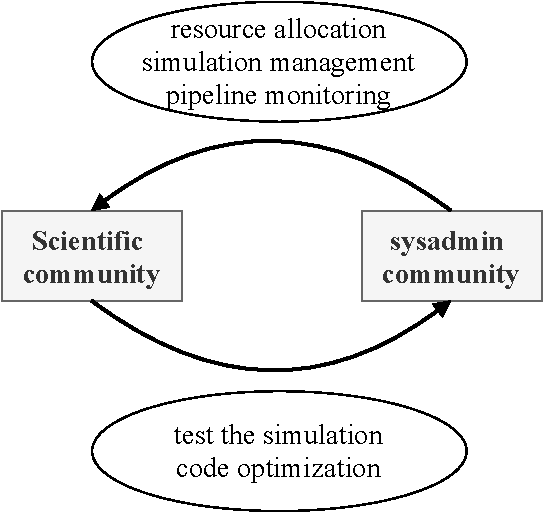
\includegraphics[scale=0.75]{figs/scientific_sysadmin_optimization.pdf}}
\caption{A basic relationship between the scientific community that issues simulations to be executed on the computing resources, and the system administration team that deals with process allocation, execution, and management of resources. The continuous improvements between the two communities involve the steps indicated next to the arrows.}
\label{community-optimization}
\end{figure}

\par Unfortunately, there will always be moments when the sysadmin team that is monitoring a particular computing node (e.g., cluster, server racks, etc.) cannot keep track of the \emph{health status} of the entire architecture at all times (although recently, some interesting models emerged within the literature that could improve the machine health status \cite{hasani2019machine,lin2020health} in an automated way). In order to properly, securely, and efficiently maintain a large-scale server infrastructure up and running (as the one that is present in a physics research department), there must be some kind of \emph{alert system} that is constantly analyzing the system resources and tries to identify unusual behavior. When a potential malfunction is identified, the core feature of the alert system is to inform the sysadmins with regards to the occurring issue(s).
\par In the present work, such a model is implemented; namely, a service that analyzes the logs generated by the system resources of a computing cluster (i.e., CPU usage, RAM usage, and so on) and compares the values with predefined thresholds decides if the monitored values indicate some unusual behavior. If indeed, the thresholds are exceeded, the service will immediately raise an alert, sending information with the occurring issue to the sysadmin teams, which then can take action.
\par The paper is organized as follows: in Section \ref{section-introduction}, a brief introduction of system administration is made, with motivation for implementing an alert system within large-scale computing infrastructure. Furthermore, in Section \ref{section-alert-workflow} the general overview on how the \emph{pythonic} implementation of the current research actually works, mentioning its main features and advantages. Section \ref{section-data-ingest} discusses the services that are used in order to keep track of changes within the log-files generated by the system resources, while Section \ref{section-thresholds} presents the method of deciding between \emph{normal} and \emph{unusual} behavior of said resources. Finally, an overview of the implementation which sends the actual alerts to the sysadmin team (via email) is made in Section \ref{section-email-alert}, followed up by some concluding remarks and potential improvements of the project itself, given in Section \ref{section-conclusions}.

\section{Alert-System Workflow}
\label{section-alert-workflow}
Implementation of the alert system is quite straightforward, following a procedure that does not require too much information. Fig. \ref{alert-system-general-workflow} shows how the process of taking action (i.e., fixing occurring issues on the computing nodes) by the administration team is taking place. Usually, the personnel that deal with system administration is located on-site, since the need-of-action would sometimes require physical access on the barebone servers. However, considering the current pandemic situation \cite{ciotti2020covid}, the paradigm has shifted a lot to remote work, with the possibility of remote access by the sysadmins \cite{sallow2020client} to any computing cluster located in the departments they monitor. As a result, the alert system will eventually inform both groups, and depending on the type of issue encountered, actions will be made by one or the other (or even both).
\par The reason behind choosing \emph{Python} \cite{python3} as the development tool here lies in its overall great compatibility with different operating systems, consistency between different system architectures (e.g., x86, ARM, \cite{blem2013power}), well-documented resources, robust packages that allow the implementation of all the required instructions securely and reliably.
\par Between the monitoring phase and the alert + action phases, the current approach involves three major stages:
\begin{description}
    \item[\emph{Step0 - Service configuration}] $\\$ This is done before the alert system is turned on, by setting some parameters to the desired values. The sysadmin team must decide on their values, depending on the required regime of execution. Discussion on the parameters will be made throughout the paper.
     \item[Stage-1 - \emph{Data ingest}] $\\$ This is the first step, in which the implemented service is extracting the data coming from the computing resources. These data contain information with regards to the state of each resource, the status of all the running processes, and so on. They usually come in form of \emph{log files}. Incoming data is stored at a fixed path, and the alert service will check for changes within those files.
     \item[Stage-2 - \emph{Log analysis}] $\\$ With the incoming data from the monitored machines finally read, the service will analyze them in terms of their numerical values, i.e., for each system stat (CPU usage, RAM usage, incoming/outgoing network traffic). The stats of interest will be compared with the \emph{thresholds}, which dictate whether the resources behave under normal or unusual conditions.
     \item[Stage-3 - \emph{Alerts}] $\\$ If the monitored resources show that indeed their behavior is unusual (considering any of the controlled stats), the python implementation will trigger a so-called \emph{alert}: a chain of procedures that follow the set of parameters defined in \emph{Step0} which will inform sysadmins with regards to the encountered issue. The process of informing the sysadmin teams is done via email \cite{postel1982rfc0821}. Its ease-of-use and ease-of-access allow the members to quickly and efficiently be informed, since the e-mail clients can run on pretty much any device (from a personal computer to a laptop, tablet, and smartphone), becoming a great solution in the current work.
\end{description}
 
\begin{figure}[htbp]
    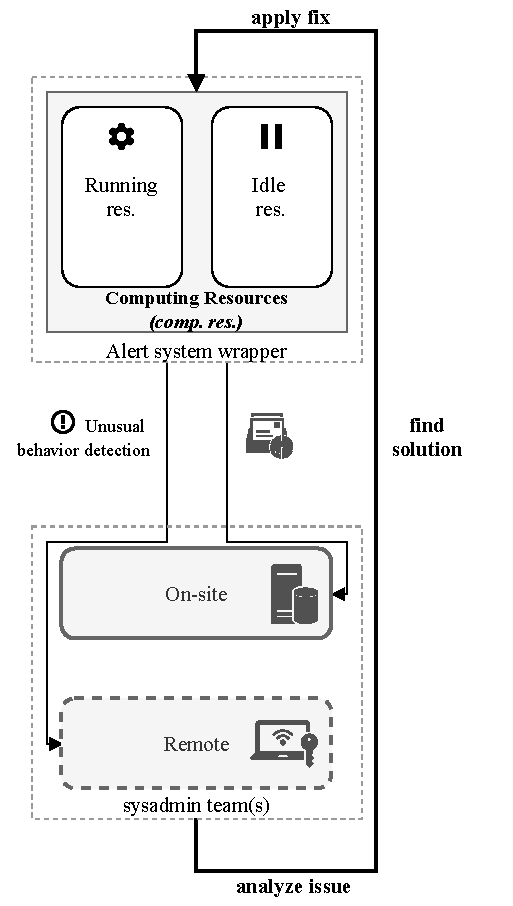
\includegraphics[scale=1.1]{figs/alert_system_improvements_v2.pdf}
    \caption{The general workflow of a system administration team, when an alert system would be deployed on the computing resources that need to be monitored.}
    \label{alert-system-general-workflow}
\end{figure}

\par Now that the core stages of the implementation were sketched (see also Fig. \ref{fig-operation-mode} for a graphical representation that encapsulates its features), it is instructive to describe each stage in particular, with its main goals and characteristics.

\begin{figure}[htbp]
    \centering
    % 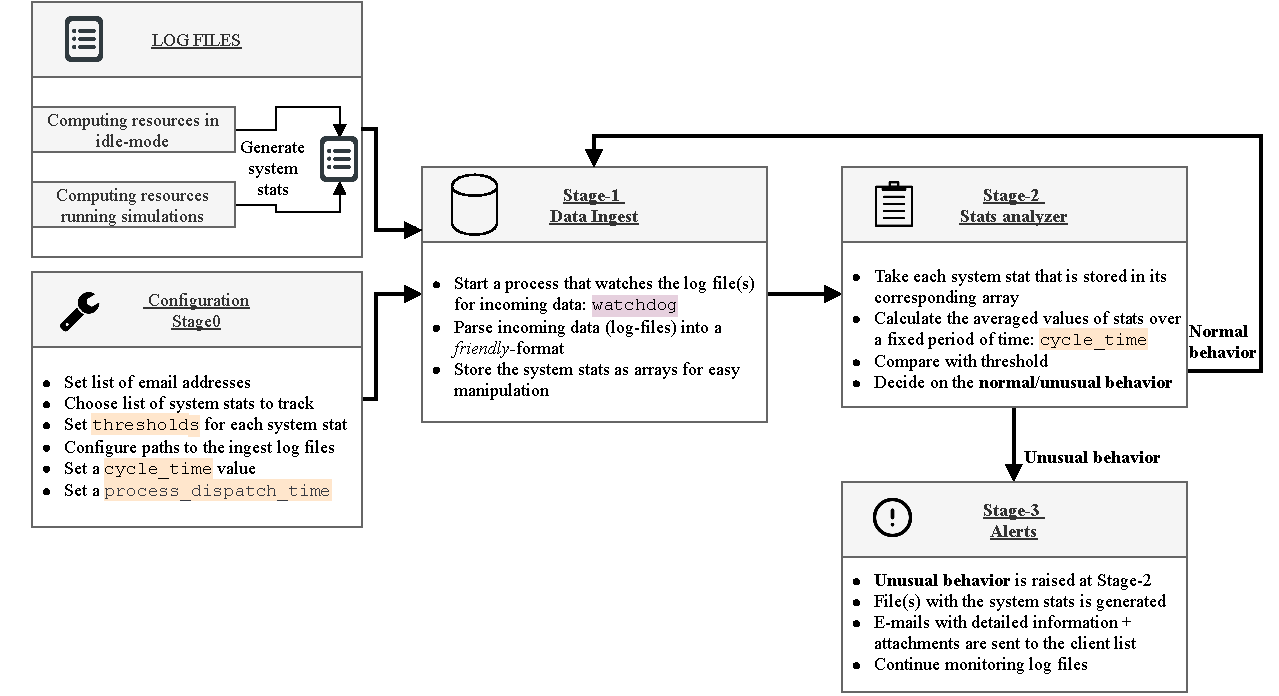
\includegraphics[width=1.0\textwidth]{figs/alert_system_operation_mode.pdf}
    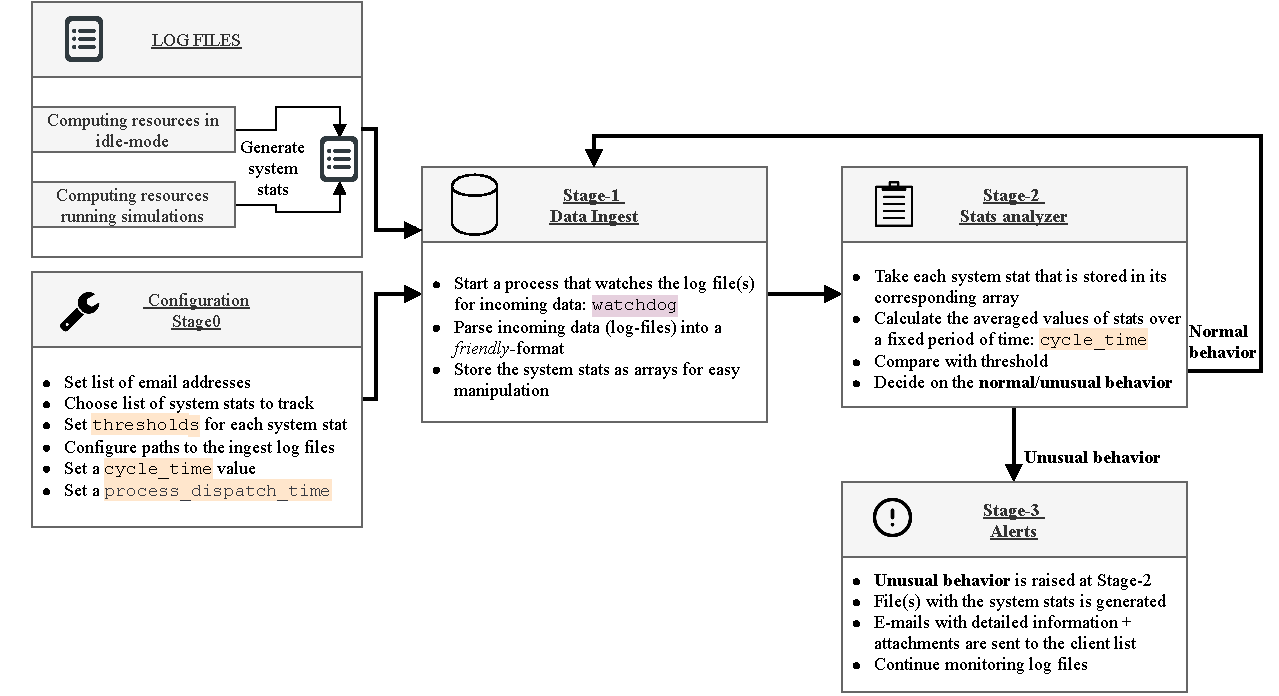
\includegraphics[scale=0.2]{figs/alert_system_operation_mode.pdf}
    \caption{Complete overview of the 3-stage operation mode of the alert implementation. Details on the marked variables are describe throughout the paper.}
    \label{fig-operation-mode}
\end{figure}

\section{Watchdog - Data ingest}
\label{section-data-ingest}

It was already mentioned that one can consider the underlying computing infrastructure as being composed of two types of resources: 1) the computing nodes that execute jobs (i.e., numerical simulations) and 2) the idling resources (i.e., nodes that wait for additional jobs picked-up by the resource management tool and allocated on the job pool by the sysadmins).
\par Both resource groups are required to send information related to their current status to the alert system. When dealing with large-scale systems, each node on the cluster must send its corresponding system stats, usually under the form of a log file. An easy way of assuring that all the nodes send their information to a centralized "master node" is by using a so-called \emph{log shipper}. One great example is the Filebeat \cite{filebeat} service, which collects system information and ships it as a log file via the network to any client. In fact, in a previous research \cite{poenaru-elk}, an implementation that can deliver logs via Filebeat was tested for multiple machines. The "master node" consists of a central machine that collects all the logs coming from the entire computing infrastructure, with each log file usually updating very often. The alert service is also deployed on the master node (so far it was tested as a python script that is running in the background, as a process).
\par With all the logs from each computing node saved in a centralized location, the \emph{python watcher} - part of Stage 1 - can monitor those files continuously. In the current testing procedures, new log data arrived (on average) each 2-3 seconds. Since the log files are constantly changed and overwritten by newly ingested data, it is required that the files must be read again and again by the python service. This is done via the \texttt{watchdog} package \cite{watchdog}. With the help of this python module, one can take a list of log files, create a set of \emph{file system handlers} wrapped into an \texttt{Observer} class, and then the implementation starts to "watch" every file within the list, keeping track of every new \emph{event} that arrives within any of the files. An event is represented by a trigger of the type \texttt{file\_modified}, meaning that once a file has some new content in it, its state is modified, and as such, the file event handler returns the newly modified state. By default, the \texttt{Observer} class comes with some predefined methods that must be used within the alert system. \texttt{start()} is called before all other steps within the multi-stage pipeline. The methods \texttt{stop()} and \texttt{join()} are used once no other log entries are arriving in the corresponding paths (signaling that there could be issues with the connection, or the Filebeat service failed within the computing cluster). Listing \ref{watchdog-code} shows a basic example of a method that checks for new events in a file, as long as no keyboard keys are pressed.

\begin{lstlisting}[language=Python, caption=A straightforward example of using the watchdog module to track a file for any changes.,basicstyle=\footnotesize,label={watchdog-code}]
 event_handler = LoggingEventHandler()
    observer = Observer()
    observer.schedule(event_handler, path, 
                            recursive=True)
    observer.start()
    try:
        while True:
            time.sleep(1)
    except KeyboardInterrupt:
        observer.stop()
    observer.join()
\end{lstlisting}

In the current implementation, the watchdog module is monitoring a set of log files in which content is written constantly, then with the help of the so-called \texttt{Reader} class, the incoming log data is parsed and stored in memory as arrays (the arrays are cleared every once in a while to avoid any memory overhead).

\section{Thresholds - normal vs. unusual behavior}
\label{section-thresholds}

With the arrays generated in Stage-1, it is possible to go into Stage-2, where some numerical analysis is performed on the collected data. This is a crucial step since it involves deciding if any of the incoming stats for a particular computing node is expecting normally or not.
\par The decision between normal vs. expected behavior on a system stat is taken by comparing its averaged value over a fixed period of time. The fixed period is configured within Stage-0 (i.e., the \texttt{cycle\_time}) by the user (sysadmin). Then, within a \texttt{cycle\_time}, every new log data that arrives at the master node is collected by the watcher (via the \texttt{Observer()} and its file event handler), added in its corresponding array (denoted by "stack" within the code-base). After a \texttt{cycle\_time} has passed, the filled arrays (stacks) are analyzed. As an example, for the CPU usage and RAM usage, the corresponding functions that perform numerical analysis are defined below (see Listing \ref{analyse-code}). Due to the space constraints of the current paper, further examples will only focus on the CPU usage and the RAM (memory) usage within the system resources.

\begin{lstlisting}[language=Python, caption=The methods for calculating averaged stats values used within the project code-base.,basicstyle=\footnotesize,label={analyse-code}]
@classmethod
    def Analyze_CPU_Usage_Stack(cls, 
                cpu_usage_stack, cpu_threshold):
 @classmethod
    def Analyze_MEM_Usage_Stack(cls,
                mem_usage_stack, mem_threshold):
\end{lstlisting}

With the obtained average values for each stat (e.g, CPU usage, RAM usage), the next step is to compare them with the \texttt{thresholds}. Within the code-base, they are declared as a dictionary (see Listing \ref{thresholds}).

\begin{lstlisting}[language=Python, caption=Declaration of some thresholds within the code-base.,basicstyle=\footnotesize,label={thresholds}]
    thresholds = {"cpu": 75,
                  "mem": 75}
\end{lstlisting}

In the example shown in Listing \ref{thresholds}, both the CPU and the RAM usage upper limit were set to 75, meaning that if within a \texttt{cycle\_time}, any monitored node that exceeds these limits (e.g., the CPU usage or RAM usage - or both - are higher than $75\%$)  will raise the \emph{unusual behavior}. Obviously, if the conditions for exceeding the upper limit are not met, the computer nodes are considered to behave as expected (normal behavior).
\par As Fig. \ref{fig-operation-mode} shows, this is the crucial step in deciding whether the alert via e-mail stage should be called or not. Under normal behavior of the monitored nodes, after each \texttt{cycle\_time} the arrays are cleared, and the watcher module continues to read new log entries.

\section{Alert via email}
\label{section-email-alert}

The last step in the implementation is the actual alert itself, which is informing the sysadmins with regards to some detected unusual behavior, and this is done by e-mail to a list of clients (each client represents a member of the sysadmin team and it requires a valid e-mail address). As already mentioned at the beginning of Section \ref{section-alert-workflow}, the choice of an e-mail based alert system was simply because of reliability and convenience (no extra apps or web services required).
\par In terms of required packages, the following python modules are used \cite{emails}:
\begin{itemize}
    \item \texttt{smtplib}
    \item \texttt{ssl}
    \item \texttt{email.mime.base.MIMEBase}
    \item \texttt{email.mime.text.MIMEText}
    \item \texttt{email.mime.text.MIMEMultipart}
\end{itemize}

The built-in Python module \texttt{smtplib} \cite{smtplib} allows one to send e-mails using the well-known SMTP protocol (Simple Mail Transfer Protocol). The module uses the standard protocol that was developed a long time ago by \cite{postel1982rfc0821}.
\par It is worth mentioning certain characteristics of the current approach. The e-mails are sent through a Gmail account that was created for \emph{Development}, turning on the feature \emph{Less secure app access} \cite{less-secure}. This way, the implemented algorithm can send e-mails securely to a list of clients.
\par In the code-base shown in Listing \ref{message-header}, the address that is used for sending alerts is configured, together with the list of clients that should receive the alert and a subject.

\begin{lstlisting}[language=Python, caption={Setting up the e-mail headers, such as the destination and subject.},basicstyle=\footnotesize,label={message-header}]
 message = MIMEMultipart()
        message["From"] = ROOT_EMAIL
        
        message["To"] = email_address
        message["Subject"] = 
            f'{str(datetime.utcnow())[:19]}
            - Alert via DFCTI Monitoring System'
\end{lstlisting}

With the subject properly configured, the next step is to create the attachments that will be added to the final message. The attachments consist of graphical representations (done with the \texttt{matplotlib} package \cite{hunter2007matplotlib}) with the system resources which raised unusual behavior (in Listing \ref{create-email} it is denoted by \text{part2}). For example, if one of the nodes has an unusually large CPU usage, then a plot with the CPU usage within the last \texttt{cycle\_time} time-interval is plotted and compared with the threshold. Another attachment is a file that contains all the numerical data with the recorded logs (within the code-base shown in Listing \ref{create-email} it is the "dat" file denoted by the variable \texttt{part1}).

\begin{lstlisting}[language=Python, caption={Create attachments and save them securely by encoding them and embed them as string objects within the final object.},basicstyle=\footnotesize,label={create-email}]
# Adding the body to the actual email
message.attach(MIMEText(message_body, "plain"))

# Open the dat file in binary mode
with open(attachment_files[0], "rb") as attachment:
    # Add file as application/octet-stream
    part1 = MIMEBase("application", "octet-stream")
    part1.set_payload(attachment.read())

    # Open the plot file in binary mode
with open(attachment_files[1], "rb") as attachment:
    # Add file as application/octet-stream
    part2 = MIMEBase("application", "octet-stream")
    part2.set_payload(attachment.read())

# Encode file in ASCII characters to send by email
encoders.encode_base64(part1)
encoders.encode_base64(part2)

# Add header as key/value pair to attachment part
part1.add_header(
    "Content-Disposition",
    f"attachment; filename= {attachment_files[0]}",)

# Add header as key/value pair to attachment part
part2.add_header(
    "Content-Disposition",
    f"attachment; filename= {attachment_files[1]}",)

# Add attachment to message +
# convert message to string
message.attach(part1)
message.attach(part2)

final_alert = message.as_string()
\end{lstlisting}

With the alert message properly constructed, the last step is to send it securely to the client list. This is done by opening an \texttt{ssl} connection. The code example sketched in Listing \ref{ssl-email} creates a secure connection with Gmail’s SMTP server, using the \texttt{SMTP\_SSL()} of \texttt{smtplib} to initiate a TLS-encrypted connection \cite{emails}. The default context of \texttt{ssl} validates the hostname and its certificates and optimizes the security of the connection.

\begin{lstlisting}[language=Python, caption={Procedure for sending the e-mail securely, through \textit{ssl}. The dotted code-base marks some debug steps that are irrelevant to the current discussion.},basicstyle=\footnotesize,label={ssl-email}]
CONTEXT = ssl.create_default_context()
with smtplib.SMTP_SSL("smtp.gmail.com", 
            PORT, context=CONTEXT) as mail_server:
    time_stamp = str(datetime.utcnow())[0:19]
    # log-in stage
    try:
        mail_server.login(ROOT_EMAIL, UNICORN_ID)
    except Exception as exc:
        ...
    else:
        ...
    # sending stage
    try:
        mail_server.sendmail(ROOT_EMAIL, 
                    email_address, final_alert)
    except Exception as exc:
        ...
    else:
        ...
\end{lstlisting}

With the code-base complete (Listings \ref{message-header}-\ref{create-email}-\ref{ssl-email}), in case of any unexpected behavior detected within the monitoring process, alerts will be constantly sent to the sysadmin team. Examples of e-mails that can be received are shown in Fig. \ref{emails-pics}. Fig. \ref{cpu-ss} shows the plot with the CPU usage for a node that has unexpected behavior.

\begin{figure*}[htbp]
    \centering
    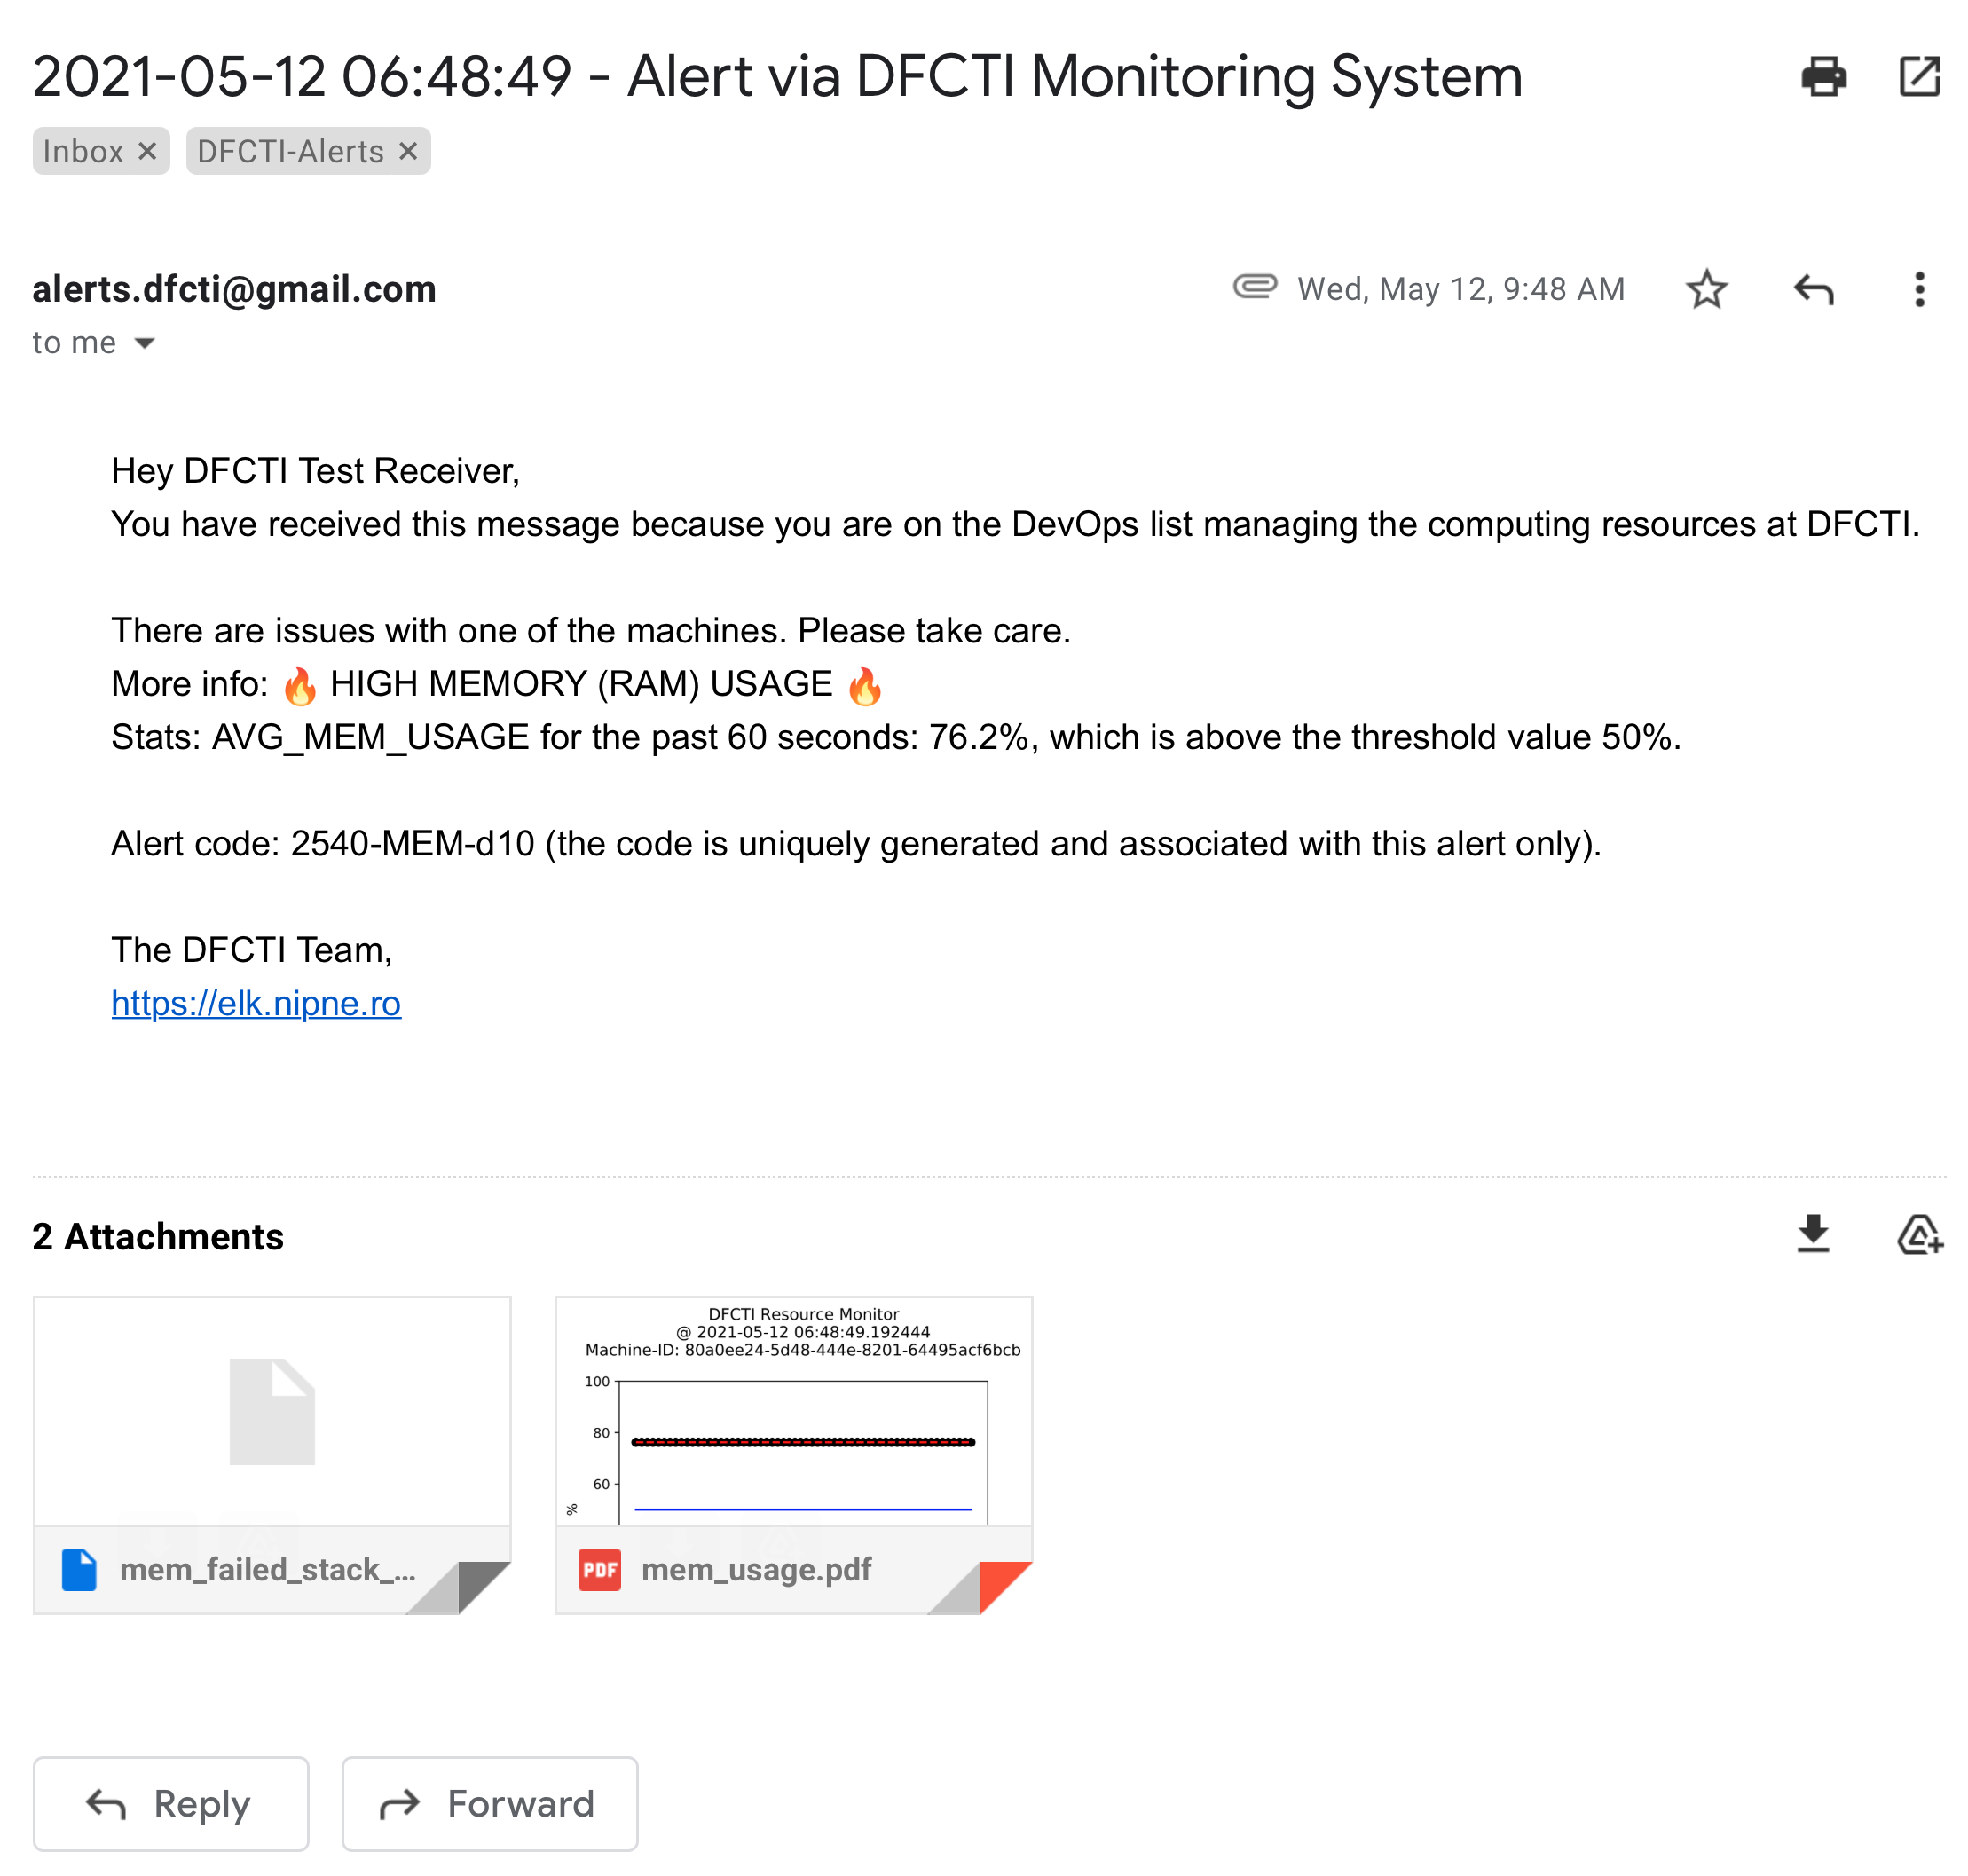
\includegraphics[scale=0.4]{figs/example_usecase_ram.png}
    \caption{Example of an alert that is sent when RAM usage behaves in an unusual manner. The two attachments can also be seen in the bottom of the screenshot}
    \label{emails-pics}
\end{figure*}

\begin{figure*}[htbp]
    \centering
    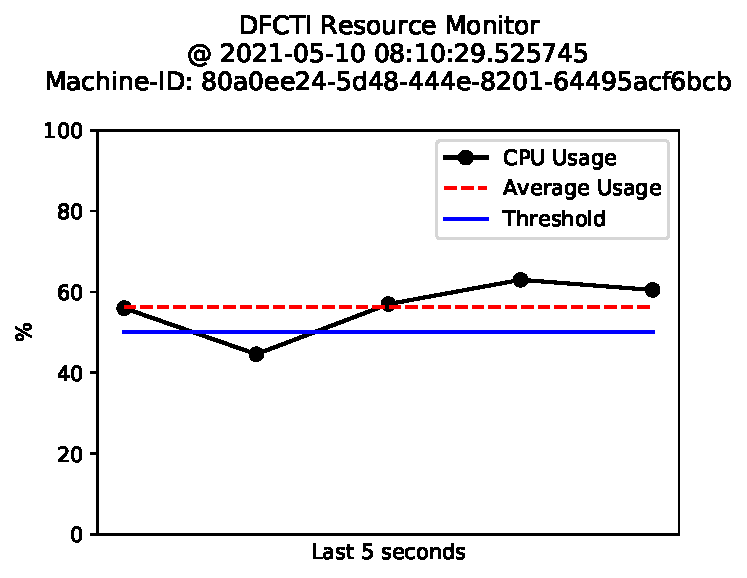
\includegraphics[scale=0.6]{figs/cpu_usage.pdf}
    \caption{The plot file within the attachments for an alert which informs the sysadmins on high CPU usage of a particular node (the unique \texttt{machine-id} corresponds to that node).}
    \label{cpu-ss}
\end{figure*}

\section{Conclusions \& Future Work}
\label{section-conclusions}

In this work, a description of the development process for an alert system was made. The importance of a system administration team that assures efficient resource management was illustrated in the beginning. The alert system consisted of several stages of procedures that were incorporated in a general workflow which performed the constant monitoring of a set of log files, then perform numerical analysis on the parsed log data, compare each system stat with the configured thresholds, decide on the normal/unusual behavior of each compute resource within the infrastructure, and then finally, create an automated e-mail message containing i) detailed text with the detected "anomaly" and ii) attachment files with graphical representations and tabulated data.
\par The current code-base used only open-source modules developed excursively in Python, assuring in this way a great degree of compatibility with most system architectures, operating systems, and environment type (i.e., bare-bone, virtualized). Moreover, the scalability of Python allows the current implementation to be deployed on large-scale clusters even through containerized approaches (i.e., Docker \cite{merkel2014docker}, K8s \cite{brewer2015kubernetes}). In fact, this is a major next step in the development process of the project.
\par Through the \texttt{watchdog} module, it was possible to monitor log files that receive new data constantly. The \texttt{smtplib} and \texttt{email} modules allowed for establishing secured connections to the Gmail server, encode files as attachments and finally send the final message (saved as a string object) to an entire list of e-mail addresses. The e-mails are sent securely, using the SSL/TLS protocols. The entire code-base is publicly available on GitHub \cite{github-codebase}.
\par The relationship between the scientific community and the sysadmin community within a research department was illustrated in the Introduction, emphasizing the reciprocal improvement cycle between the two, when proper actions are made on both sides.
\par With the current implementation, a sysadmin team will be able to have uninterrupted resource management and monitoring for the entire computing infrastructure, being able to quickly take action on the identified issues. By taking the proper actions on the computing resources (either the idle ones or the ones which execute jobs) an efficient pipeline is created, resulting in an optimal run-time of existing jobs, but also a proper execution of new incoming jobs.

% \subsection{Figures and Tables}
% \paragraph{Positioning Figures and Tables} Place figures and tables at the top and 
% bottom of columns. Avoid placing them in the middle of columns. Large 
% figures and tables may span across both columns. Figure captions should be 
% below the figures; table heads should appear above the tables. Insert 
% figures and tables after they are cited in the text. Use the abbreviation 
% ``Fig.~\ref{fig}'', even at the beginning of a sentence.
% \begin{table}[htbp]
% \caption{Table Type Styles}
% \begin{center}
% \begin{tabular}{|c|c|c|c|}
% \hline
% \textbf{Table}&\multicolumn{3}{|c|}{\textbf{Table Column Head}} \\
% \cline{2-4} 
% \textbf{Head} & \textbf{\textit{Table column subhead}}& \textbf{\textit{Subhead}}& \textbf{\textit{Subhead}} \\
% \hline
% copy& More table copy$^{\mathrm{a}}$& &  \\
% \hline
% \multicolumn{4}{l}{$^{\mathrm{a}}$Sample of a Table footnote.}
% \end{tabular}
% \label{tab1}
% \end{center}
% \end{table}

\section*{Acknowledgment}

This work was done within the Department of Computational Physics and Information Technology at \emph{Horia Hulubei} National Institute of Physics and Nuclear Engineering. The development was funded by the European Regional Development Fund through project CECBID-EOSC (POC/397/1/1-124405).

\bibliographystyle{unsrt}
\bibliography{references}

\end{document}
